\section{Convolutional Neural Networks}
Convolutional neural networks are the tools for performing most of the visual tasks, like classification and detection, and they are probably the most widely known deep learning model. 
%(sta facendo un recap tipo? manca una lezione forse?)

\subsection{The Feature Extraction Perspective}
Instead of just feeding directly our image to a classifier, we perform some preliminary step to extract features from the images, we will perform some preliminary algorithm that maps our image into a vector which is informative for defining the label where the image belongs to. You are not trying to directly handle the image has a vector but you extract some meaningful information out of the image in order to feed this additional information to a standard classifier. Feature extraction is a winning strategy, for example it lets you embed some a-priori additional information you have on your data. One way is to do exploratory data -analysis and to draw some rule from what comes out, identifying the various classes by some rule based feature; the problem with this kind of features is that is difficult to design complex relations which involve many variables in which sometimes it's not easy to separate the variables. Neural networks and things like SVM on the other side are able to learn more complex relationships among variables that include many variables. An option is to add hand written features that come from our expertise to the neural network. For natural images, the hand crafted approach doesn't work and you have to go to the data driven approach. This means using Convolutional Neural Networks. Before using CNN, we need to understand how convolution works.

\subsection{Convolution}
Convolution it's, up to some change of sign, exactly as \textit{correlation}. Convolution is a linear transformation applied to an image.
\begin{center}
    $T[I](r, c)=\sum_{(x, y) \in U} w(x, y) * I(r-x, c-y)$
\end{center}
If you have an image and a filter (which is nothing more but a small image); we can consider the weights as a filter $H$ and the filter entirely defines the convolution, which operates the same in each pixel:
\begin{center}
    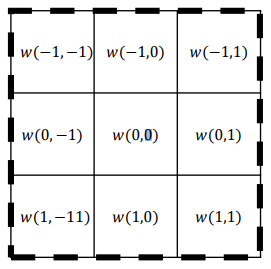
\includegraphics[width=0.3\textwidth]{images_CNN/filter.PNG}\par\vspace{1cm}
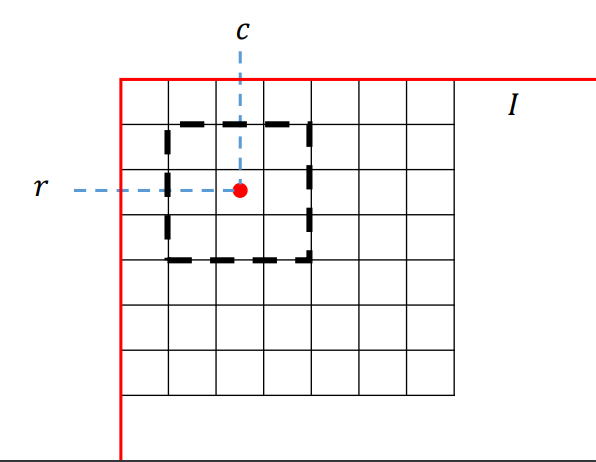
\includegraphics[width=0.45\textwidth]{images_CNN/imag.PNG}\par\vspace{1cm}
\end{center}

The convolution of the input image against this filter is still an image. The size of the output image in principal should be the same of the input one. The same operation is performed in each pixel of the input image and we get a value for each pixel, which is gonna be just the linear combination of the pixel values in a neighbor of the pixel (which has the same size of the pixel).\\
So you take your filter, you place it over the image right in the position where you want to compute the output (in this case you place the filter so that the center goes in $(r,c)$) and the output is the linear combination of the pixel values using these coefficients as weights for the linear combination. \\
Convolution is the process of adding each element of the image to its local neighbors, weighted by the kernel. What happens on boundaries?\\
There are different options; the simplest thing is to use 0 padding, so you set 0s where the filter goes out of the image (so its black), otherwise you can compute the output of the convolution only at those pixels where the filter can be entirely included in the image. Note that a minus sign means that you have to flip your image, it's exactly the same if you flip your filter, it's important only if you define the filters but in general we will learn the $w$. Convolution was already used in signal processing, it's used to compute the Fourier transformed, it wasn't invented for neural networks. \\
Correlation is the same but in correlation you have the plus sign whether in convolution you have the minus sign. 
%(inizia a fare esempi a caso)

\subsection{CNN Layers}
CNN are networks that take as input an image and provide as output as any neural networks, for example for classification, a set of probabilities associated to each class. For example, for the CIFAR dataset we take as input 32x32x3 images and we provide as output 10 values which are the posterior probabilities over the 10 classes. In a CNN you see some structure of the image which is preserved, you see the feature maps. As you move deeper you see 
%(guarda slide) 
that they are increasing in number an decreasing in size, each of this images are layers of the volume; feature maps become smaller but deeper so the height and width of the volume decrease whether the dimension increases. In order to perform this operation that reduces the size and increases the dimension, you use 3 different layers: 

\begin{itemize}
    \item convolutional layers
    \item activation functions
    \item pooling layers, in particular max pooling
\end{itemize}

\subsubsection{Convolutional Layers}
In a CNN you have a set of filters given for each layer and these filters represent the network parameters. Let's see what is the output of the convolution of this image against a filter which is, for example, 3x3x3:

\begin{center}
    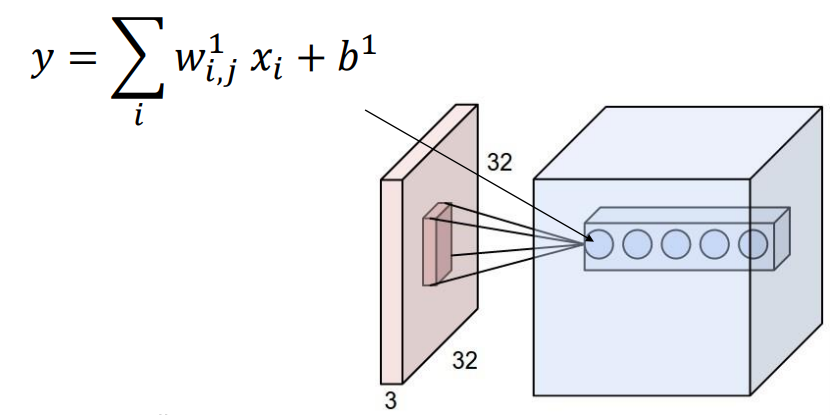
\includegraphics[width=0.5\textwidth]{images_CNN/clayers.PNG}\par
\end{center}
Remember that each filter has to have the same depth as the input volume, in this case you have 3 channels so the filter will be 3x3x3. Each pixel in the output image is gonna be given by the filter and the pixel values of your image in a neighbor of the same pixel, as we saw before. What we have in that point 
%in the image 
are the weights $w$ multiplied by the input $x_{i}$ plus some bias, it's a linear combination. You compute different filters and the output images becomes deeper. Increasing the depth is done simply by adding multiple filters; the parameters of a convolutional layer are all the weights that are stored in filters plus one bias associated to each filter.

%As you can see in the next slides,
As you can imagine, one input image with one filter gives one output map, two filters give two output maps etc. The important thing is that the filter has to have the same depth as the input map, and the filter is applied to the whole spatial extent of the input, and adding more filters increases the number of output maps.

If you feed a network with 3 input maps, what happens is that all your filter will be 3 different layers and the filters corresponding to the moving output map are those that are also moving. How many parameters does this layer have?
\begin{center}
    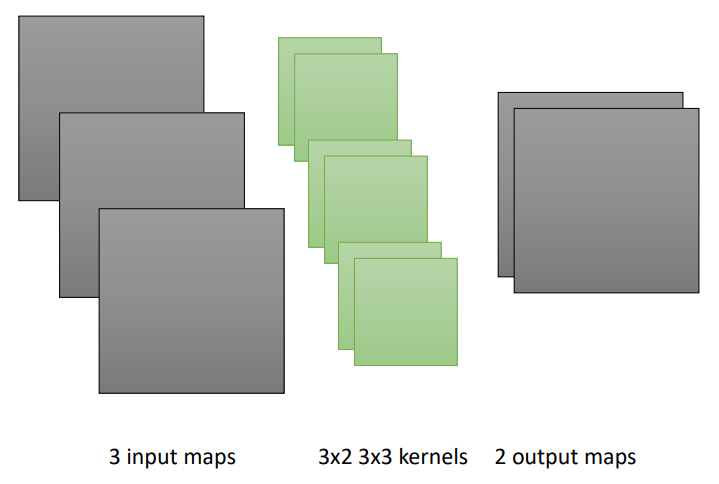
\includegraphics[width=0.5\textwidth]{images_CNN/layers.PNG}\par
\end{center}
Each layer has 9 parameters (3x3), but each filter has 3 layers so its 9x3=27 for each filter, x2=54; moreover you have to consider the bias, one for each filters. So: 54 for the filters + 2 biases = 56 trainable parameters. What's really important is that convolution mixes all the input channels. Typically you have small filters in these networks, they have a negligible size w.r.t. the image size.

\subsubsection{Activation Functions}
Convolutional layers perform linear combinations, so what you get at the end is again a linear combination. Like in the multilayer perceptron, you have to introduce some non-linearity and you do this with the activation function, otherwise the CNN would be equal to a linear classifier. The most popular is the Rectified Linear Unit (RELU):
\begin{center}
    $T(x)=\left\{\begin{array}{ll}{x,} & {\text { if } x \geq 0} \\ {0,} & {\text { if } x<0}\end{array}\right.$
\end{center}
Another option is a variant of the RELU called leaky RELU:
\begin{center}
    $T(x)=\left\{\begin{array}{ll}{x,} & {\text { if } x \geq 0} \\ {0.01 * x} & {\text { if } x<0}\end{array}\right.$
\end{center}
These functions activates the neurons performing some thresholding on the feature maps. Other options are:


\subsubsection{Pooling Layers}
These layers reduce the spatial extent of the input volume. The most popular is the MaxPooling layer which operates independently on each slice. 
\begin{center}
    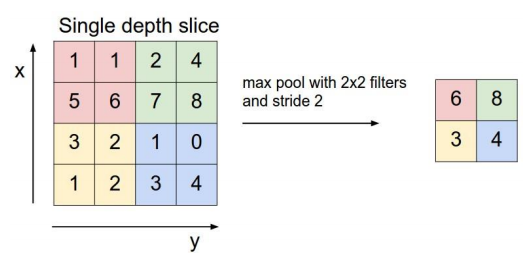
\includegraphics[width=0.5\textwidth]{images_CNN/maxpool.PNG}\par
\end{center}

\subsubsection{Fully Connected Layer}
When you get to the end reducing the spatial extend with the pooling layers, what you get is that your volume will have a special extent equal to 1, so it's just a large vector. This vector is the feature vector and with it you train a multilayer perceptron, which is called a fully connected layer.

\vspace{1cm}

The first CNN goes back to 1998, the LeNet-5. After that NN were forgotten for a while until a CNN model won the ImageNet competition of 2012, AlexNet, which was the first deep CNN. There are two main reasons for which they had difficulties in spreading after 1998: heavy computation and lack of data. Moving to these days, a lot of things have changed: on one side new mosfet technologies, fast CPU, graphic computation, on the other side amazingly increasing data of all kinds are created each second. These two factors, parallel fast computing and a lot of training data, really played a crucial role for the escalation of neural networks.